\FChapter{Chapter Four}{3}

\Lettrine{F}{rom} \textsc{my discourse} with \Mr{} Lloyd, and from the above reported conference
between Bessie and Abbot, I gathered enough of hope to suffice as a
motive for wishing to get well: a change seemed near,---I desired and
waited it in silence. It tarried, however: days and weeks passed: I had
regained my normal state of health, but no new allusion was made to the
subject over which I brooded. \Mrs{} Reed surveyed me at times with a
severe eye, but seldom addressed me: since my illness, she had drawn a
more marked line of separation than ever between me and her own
children; appointing me a small closet to sleep in by myself, condemning
me to take my meals alone, and pass all my time in the nursery, while my
cousins were constantly in the drawing-room. Not a hint, however, did
she drop about sending me to school: still I felt an instinctive
certainty that she would not long endure me under the same roof with
her; for her glance, now more than ever, when turned on me, expressed an
insuperable and rooted aversion.

Eliza and Georgiana, evidently acting according to orders, spoke to me
as little as possible: John thrust his tongue in his cheek whenever he
saw me, and once attempted chastisement; but as I instantly turned
against him, roused by the same sentiment of deep ire and desperate
revolt which had stirred my corruption before, he thought it better to
desist, and ran from me tittering execrations, and vowing I had burst
his nose. I had indeed levelled at that prominent feature as hard a
blow as my knuckles could inflict; and when I saw that either that or my
look daunted him, I had the greatest inclination to follow up my
advantage to purpose; but he was already with his mama. I heard him in
a blubbering tone commence the tale of how \enquote{that nasty Jane
	Eyre} had flown at him like a mad cat: he was stopped rather harshly---

\enquote{Don't talk to me about her, John: I told you not to go near
	her; she is not worthy of notice; I do not choose that either you or
	your sisters should associate with her.}

Here, leaning over the banister, I cried out suddenly, and without at
all deliberating on my words---

\enquote{They are not fit to associate with me.}

\Mrs{} Reed was rather a stout woman; but, on hearing this strange and
audacious declaration, she ran nimbly up the stair, swept me like a
whirlwind into the nursery, and crushing me down on the edge of my crib,
dared me in an emphatic voice to rise from that place, or utter one
syllable during the remainder of the day.

\enquote{What would Uncle Reed say to you, if he were alive?} was my
scarcely voluntary demand. I say scarcely voluntary, for it seemed as
if my tongue pronounced words without my will consenting to their
utterance: something spoke out of me over which I had no control.

\enquote{What?} said \Mrs{} Reed under her breath: her usually cold
composed grey eye became troubled with a look like fear; she took her
hand from my arm, and gazed at me as if she really did not know whether
I were child or fiend. I was now in for it.

\enquote{My Uncle Reed is in heaven, and can see all you do and think;
	and so can papa and mama: they know how you shut me up all day long, and
	how you wish me dead.}

\Mrs{} Reed soon rallied her spirits: she shook me most soundly, she boxed
both my ears, and then left me without a word. Bessie supplied the
hiatus by a homily of an hour's length, in which she proved beyond a
doubt that I was the most wicked and abandoned child ever reared under a
roof. I half believed her; for I felt indeed only bad feelings surging
in my breast.

November, December, and half of January passed away. Christmas and the
New Year had been celebrated at Gateshead with the usual festive cheer;
presents had been interchanged, dinners and evening parties given. From
every enjoyment I was, of course, excluded: my share of the gaiety
consisted in witnessing the daily apparelling of Eliza and Georgiana,
and seeing them descend to the drawing-room, dressed out in thin muslin
frocks and scarlet sashes, with hair elaborately ringletted; and
afterwards, in listening to the sound of the piano or the harp played
below, to the passing to and fro of the butler and footman, to the
jingling of glass and china as refreshments were handed, to the broken
hum of conversation as the drawing-room door opened and closed. When
tired of this occupation, I would retire from the stairhead to the
solitary and silent nursery: there, though somewhat sad, I was not
miserable. To speak truth, I had not the least wish to go into company,
for in company I was very rarely noticed; and if Bessie had but been
kind and companionable, I should have deemed it a treat to spend the
evenings quietly with her, instead of passing them under the formidable
eye of \Mrs{} Reed, in a room full of ladies and gentlemen. But Bessie,
as soon as she had dressed her young ladies, used to take herself off to
the lively regions of the kitchen and housekeeper's room, generally
bearing the candle along with her. I then sat with my doll on my knee
till the fire got low, glancing round occasionally to make sure that
nothing worse than myself haunted the shadowy room; and when the embers
sank to a dull red, I undressed hastily, tugging at knots and strings as
I best might, and sought shelter from cold and darkness in my crib. To
this crib I always took my doll; human beings must love something, and,
in the dearth of worthier objects of affection, I contrived to find a
pleasure in loving and cherishing a faded graven image, shabby as a
miniature scarecrow. It puzzles me now to remember with what absurd
sincerity I doated on this little toy, half fancying it alive and
capable of sensation. I could not sleep unless it was folded in my
night-gown; and when it lay there safe and warm, I was comparatively
happy, believing it to be happy likewise.

Long did the hours seem while I waited the departure of the company, and
listened for the sound of Bessie's step on the stairs: sometimes she
would come up in the interval to seek her thimble or her scissors, or
perhaps to bring me something by way of supper---a bun or a
cheese-cake---then she would sit on the bed while I ate it, and when I
had finished, she would tuck the clothes round me, and twice she kissed
me, and said, \enquote{Good night, Miss Jane.} When thus gentle, Bessie
seemed to me the best, prettiest, kindest being in the world; and I
wished most intensely that she would always be so pleasant and amiable,
and never push me about, or scold, or task me unreasonably, as she was
too often wont to do. Bessie Lee must, I think, have been a girl of
good natural capacity, for she was smart in all she did, and had a
remarkable knack of narrative; so, at least, I judge from the impression
made on me by her nursery tales. She was pretty too, if my
recollections of her face and person are correct. I remember her as a
slim young woman, with black hair, dark eyes, very nice features, and
good, clear complexion; but she had a capricious and hasty temper, and
indifferent ideas of principle or justice: still, such as she was, I
preferred her to any one else at Gateshead Hall.

It was the fifteenth of January, about nine o'clock in the morning:
Bessie was gone down to breakfast; my cousins had not yet been summoned
to their mama; Eliza was putting on her bonnet and warm garden-coat to
go and feed her poultry, an occupation of which she was fond: and not
less so of selling the eggs to the housekeeper and hoarding up the money
she thus obtained. She had a turn for traffic, and a marked propensity
for saving; shown not only in the vending of eggs and chickens, but also
in driving hard bargains with the gardener about flower-roots, seeds,
and slips of plants; that functionary having orders from \Mrs{} Reed to
buy of his young lady all the products of her parterre she wished to
sell: and Eliza would have sold the hair off her head if she could have
made a handsome profit thereby. As to her money, she first secreted it
in odd corners, wrapped in a rag or an old curl-paper; but some of these
hoards having been discovered by the housemaid, Eliza, fearful of one
day losing her valued treasure, consented to intrust it to her mother,
at a usurious rate of interest---fifty or sixty per cent.; which
interest she exacted every quarter, keeping her accounts in a little
book with anxious accuracy.

Georgiana sat on a high stool, dressing her hair at the glass, and
interweaving her curls with artificial flowers and faded feathers, of
which she had found a store in a drawer in the attic. I was making my
bed, having received strict orders from Bessie to get it arranged before
she returned (for Bessie now frequently employed me as a sort of
under-nurserymaid, to tidy the room, dust the chairs, \etc). Having
spread the quilt and folded my night-dress, I went to the window-seat to
put in order some picture-books and doll's house furniture scattered
there; an abrupt command from Georgiana to let her playthings alone (for
the tiny chairs and mirrors, the fairy plates and cups, were her
property) stopped my proceedings; and then, for lack of other
occupation, I fell to breathing on the frost-flowers with which the
window was fretted, and thus clearing a space in the glass through which
I might look out on the grounds, where all was still and petrified under
the influence of a hard frost.

From this window were visible the porter's lodge and the carriage-road,
and just as I had dissolved so much of the silver-white foliage veiling
the panes as left room to look out, I saw the gates thrown open and a
carriage roll through. I watched it ascending the drive with
indifference; carriages often came to Gateshead, but none ever brought
visitors in whom I was interested; it stopped in front of the house, the
door-bell rang loudly, the new-comer was admitted. All this being
nothing to me, my vacant attention soon found livelier attraction in the
spectacle of a little hungry robin, which came and chirruped on the
twigs of the leafless cherry-tree nailed against the wall near the
casement. The remains of my breakfast of bread and milk stood on the
table, and having crumbled a morsel of roll, I was tugging at the sash
to put out the crumbs on the window-sill, when Bessie came running
upstairs into the nursery.

\enquote{Miss Jane, take off your pinafore; what are you doing there?
	Have you washed your hands and face this morning?} I gave another tug
before I answered, for I wanted the bird to be secure of its bread: the
sash yielded; I scattered the crumbs, some on the stone sill, some on
the cherry-tree bough, then, closing the window, I replied---

\enquote{No, Bessie; I have only just finished dusting.}

\enquote{Troublesome, careless child! and what are you doing now? You
	look quite red, as if you had been about some mischief: what were you
	opening the window for?}

I was spared the trouble of answering, for Bessie seemed in too great a
hurry to listen to explanations; she hauled me to the washstand,
inflicted a merciless, but happily brief scrub on my face and hands with
soap, water, and a coarse towel; disciplined my head with a bristly
brush, denuded me of my pinafore, and then hurrying me to the top of the
stairs, bid me go down directly, as I was wanted in the breakfast-room.

I would have asked who wanted me: I would have demanded if \Mrs{} Reed was
there; but Bessie was already gone, and had closed the nursery-door upon
me. I slowly descended. For nearly three months, I had never been
called to \Mrs{} Reed's presence; restricted so long to the nursery, the
breakfast, dining, and drawing-rooms were become for me awful regions,
on which it dismayed me to intrude.

I now stood in the empty hall; before me was the breakfast-room door,
and I stopped, intimidated and trembling. What a miserable little
poltroon had fear, engendered of unjust punishment, made of me in those
days! I feared to return to the nursery, and feared to go forward to
the parlour; ten minutes I stood in agitated hesitation; the vehement
ringing of the breakfast-room bell decided me; I \emph{must} enter.

\enquote{Who could want me?} I asked inwardly, as with both hands I
turned the stiff door-handle, which, for a second or two, resisted my
efforts. \enquote{What should I see besides Aunt Reed in the
	apartment?---a man or a woman?} The handle turned, the door unclosed,
and passing through and curtseying low, I looked up at---a black
pillar!---such, at least, appeared to me, at first sight, the straight,
narrow, sable-clad shape standing erect on the rug: the grim face at the
top was like a carved mask, placed above the shaft by way of capital.

\Mrs{} Reed occupied her usual seat by the fireside; she made a signal to
me to approach; I did so, and she introduced me to the stony stranger
with the words: \enquote{This is the little girl respecting whom I
	applied to you.}

\emph{He}, for it was a man, turned his head slowly towards where I
stood, and having examined me with the two inquisitive-looking grey eyes
which twinkled under a pair of bushy brows, said solemnly, and in a bass
voice, \enquote{Her size is small: what is her age?}

\enquote{Ten years.}

\enquote{So much?} was the doubtful answer; and he prolonged his
scrutiny for some minutes. Presently he addressed me---\enquote{Your
	name, little girl?}

\enquote{Jane Eyre, sir.}

In uttering these words I looked up: he seemed to me a tall gentleman;
but then I was very little; his features were large, and they and all
the lines of his frame were equally harsh and prim.

\enquote{Well, Jane Eyre, and are you a good child?}

Impossible to reply to this in the affirmative: my little world held a
contrary opinion: I was silent. \Mrs{} Reed answered for me by an
expressive shake of the head, adding soon, \enquote{Perhaps the less
	said on that subject the better, \Mr{} Brocklehurst.}

\enquote{Sorry indeed to hear it! she and I must have some talk;} and
bending from the perpendicular, he installed his person in the arm-chair
opposite \Mrs{} Reed's. \enquote{Come here,} he said.

I stepped across the rug; he placed me square and straight before him.
What a face he had, now that it was almost on a level with mine! what a
great nose! and what a mouth! and what large prominent teeth!

\enquote{No sight so sad as that of a naughty child,} he began,
\enquote{especially a naughty little girl. Do you know where the wicked
	go after death?}

\enquote{They go to hell,} was my ready and orthodox answer.

\enquote{And what is hell? Can you tell me that?}

\enquote{A pit full of fire.}

\enquote{And should you like to fall into that pit, and to be burning
	there for ever?}

\enquote{No, sir.}

\enquote{What must you do to avoid it?}

I deliberated a moment; my answer, when it did come, was objectionable:
\enquote{I must keep in good health, and not die.}

\enquote{How can you keep in good health? Children younger than you die
	daily. I buried a little child of five years old only a day or two
	since,---a good little child, whose soul is now in heaven. It is to be
	feared the same could not be said of you were you to be called hence.}

Not being in a condition to remove his doubt, I only cast my eyes down
on the two large feet planted on the rug, and sighed, wishing myself far
enough away.

\enquote{I hope that sigh is from the heart, and that you repent of ever
	having been the occasion of discomfort to your excellent benefactress.}

\enquote{Benefactress! benefactress!} said I inwardly: \enquote{they all
	call \Mrs{} Reed my benefactress; if so, a benefactress is a disagreeable
	thing.}

\enquote{Do you say your prayers night and morning?} continued my
interrogator.

\enquote{Yes, sir.}

\enquote{Do you read your Bible?}

\enquote{Sometimes.}

\enquote{With pleasure? Are you fond of it?}

\enquote{I like Revelations, and the book of Daniel, and Genesis and
	Samuel, and a little bit of Exodus, and some parts of Kings and
	Chronicles, and Job and Jonah.}

\enquote{And the Psalms? I hope you like them?}

\enquote{No, sir.}

\enquote{No? oh, shocking! I have a little boy, younger than you, who
	knows six Psalms by heart: and when you ask him which he would rather
	have, a gingerbread-nut to eat or a verse of a Psalm to learn, he says:
	\enquote{Oh! the verse of a Psalm! angels sing Psalms;} says he,
	\enquote{I wish to be a little angel here below;} he then gets two nuts
	in recompense for his infant piety.}

\enquote{Psalms are not interesting,} I remarked.

\enquote{That proves you have a wicked heart; and you must pray to God
	to change it: to give you a new and clean one: to take away your heart
	of stone and give you a heart of flesh.}

I was about to propound a question, touching the manner in which that
operation of changing my heart was to be performed, when \Mrs{} Reed
interposed, telling me to sit down; she then proceeded to carry on the
conversation herself.

\enquote{\Mr{} Brocklehurst, I believe I intimated in the letter which I
	wrote to you three weeks ago, that this little girl has not quite the
	character and disposition I could wish: should you admit her into Lowood
	school, I should be glad if the superintendent and teachers were
	requested to keep a strict eye on her, and, above all, to guard against
	her worst fault, a tendency to deceit. I mention this in your hearing,
	Jane, that you may not attempt to impose on \Mr{} Brocklehurst.}

Well might I dread, well might I dislike \Mrs{} Reed; for it was her
nature to wound me cruelly; never was I happy in her presence; however
carefully I obeyed, however strenuously I strove to please her, my
efforts were still repulsed and repaid by such sentences as the above.
Now, uttered before a stranger, the accusation cut me to the heart; I
dimly perceived that she was already obliterating hope from the new
phase of existence which she destined me to enter; I felt, though I
could not have expressed the feeling, that she was sowing aversion and
unkindness along my future path; I saw myself transformed under \Mr{}
Brocklehurst's eye into an artful, noxious child, and what could I do to
remedy the injury?

\enquote{Nothing, indeed,} thought I, as I struggled to repress a sob,
and hastily wiped away some tears, the impotent evidences of my anguish.

\enquote{Deceit is, indeed, a sad fault in a child,} said \Mr{}
Brocklehurst; \enquote{it is akin to falsehood, and all liars will have
	their portion in the lake burning with fire and brimstone; she shall,
	however, be watched, \Mrs{} Reed. I will speak to Miss Temple and the
	teachers.}

\enquote{I should wish her to be brought up in a manner suiting her
	prospects,} continued my benefactress; \enquote{to be made useful, to be
	kept humble: as for the vacations, she will, with your permission, spend
	them always at Lowood.}

\enquote{Your decisions are perfectly judicious, madam,} returned \Mr{}
Brocklehurst. \enquote{Humility is a Christian grace, and one
	peculiarly appropriate to the pupils of Lowood; I, therefore, direct
	that especial care shall be bestowed on its cultivation amongst them. I
	have studied how best to mortify in them the worldly sentiment of pride;
	and, only the other day, I had a pleasing proof of my success. My
	second daughter, Augusta, went with her mama to visit the school, and on
	her return she exclaimed: \enquote{Oh, dear papa, how quiet and plain
		all the girls at Lowood look, with their hair combed behind their ears,
		and their long pinafores, and those little holland pockets outside their
		frocks---they are almost like poor people's children! and,} said she,
	\enquote{they looked at my dress and mama's, as if they had never seen
		a silk gown before.}}

\enquote{This is the state of things I quite approve,} returned \Mrs{}
Reed; \enquote{had I sought all England over, I could scarcely have
	found a system more exactly fitting a child like Jane Eyre.
	Consistency, my dear \Mr{} Brocklehurst; I advocate consistency in all
	things.}

\enquote{Consistency, madam, is the first of Christian duties; and it
	has been observed in every arrangement connected with the establishment
	of Lowood: plain fare, simple attire, unsophisticated accommodations,
	hardy and active habits; such is the order of the day in the house and
	its inhabitants.}

\enquote{Quite right, sir. I may then depend upon this child being
	received as a pupil at Lowood, and there being trained in conformity to
	her position and prospects?}

\enquote{Madam, you may: she shall be placed in that nursery of chosen
	plants, and I trust she will show herself grateful for the inestimable
	privilege of her election.}

\enquote{I will send her, then, as soon as possible, \Mr{} Brocklehurst;
	for, I assure you, I feel anxious to be relieved of a responsibility
	that was becoming too irksome.}

\enquote{No doubt, no doubt, madam; and now I wish you good morning. I
	shall return to Brocklehurst Hall in the course of a week or two: my
	good friend, the Archdeacon, will not permit me to leave him sooner. I
	shall send Miss Temple notice that she is to expect a new girl, so that
	there will be no difficulty about receiving her. Good-bye.}

\enquote{Good-bye, \Mr{} Brocklehurst; remember me to \Mrs{} and Miss
	Brocklehurst, and to Augusta and Theodore, and Master Broughton
	Brocklehurst.}

\enquote{I will, madam. Little girl, here is a book entitled the
	\enquote{Child's Guide,} read it with prayer, especially that part
	containing \enquote{An account of the awfully sudden death of Martha
		G---, a naughty child addicted to falsehood and deceit.}}

With these words \Mr{} Brocklehurst put into my hand a thin pamphlet sewn
in a cover, and having rung for his carriage, he departed.

\Mrs{} Reed and I were left alone: some minutes passed in silence; she was
sewing, I was watching her. \Mrs{} Reed might be at that time some six or
seven and thirty; she was a woman of robust frame, square-shouldered and
strong-limbed, not tall, and, though stout, not obese: she had a
somewhat large face, the under jaw being much developed and very solid;
her brow was low, her chin large and prominent, mouth and nose
sufficiently regular; under her light eyebrows glimmered an eye devoid
of ruth; her skin was dark and opaque, her hair nearly flaxen; her
constitution was sound as a bell---illness never came near her; she was
an exact, clever manager; her household and tenantry were thoroughly
under her control; her children only at times defied her authority and
laughed it to scorn; she dressed well, and had a presence and port
calculated to set off handsome attire.

Sitting on a low stool, a few yards from her arm-chair, I examined her
figure; I perused her features. In my hand I held the tract containing
the sudden death of the Liar, to which narrative my attention had been
pointed as to an appropriate warning. What had just passed; what \Mrs{}
Reed had said concerning me to \Mr{} Brocklehurst; the whole tenor of
their conversation, was recent, raw, and stinging in my mind; I had felt
every word as acutely as I had heard it plainly, and a passion of
resentment fomented now within me.

\Mrs{} Reed looked up from her work; her eye settled on mine, her fingers
at the same time suspended their nimble movements.

\enquote{Go out of the room; return to the nursery,} was her mandate.
My look or something else must have struck her as offensive, for she
spoke with extreme though suppressed irritation. I got up, I went to
the door; I came back again; I walked to the window, across the room,
then close up to her.

\emph{Speak} I must: I had been trodden on severely, and \emph{must}
turn: but how? What strength had I to dart retaliation at my
antagonist? I gathered my energies and launched them in this blunt
sentence---

\enquote{I am not deceitful: if I were, I should say I loved you; but I
	declare I do not love you: I dislike you the worst of anybody in the
	world except John Reed; and this book about the liar, you may give to
	your girl, Georgiana, for it is she who tells lies, and not I\@.}

\Mrs{} Reed's hands still lay on her work inactive: her eye of ice
continued to dwell freezingly on mine.

\enquote{What more have you to say?} she asked, rather in the tone in
which a person might address an opponent of adult age than such as is
ordinarily used to a child.

That eye of hers, that voice stirred every antipathy I had. Shaking
from head to foot, thrilled with ungovernable excitement, I continued---

\enquote{I am glad you are no relation of mine: I will never call you
	aunt again as long as I live. I will never come to see you when I am
	grown up; and if any one asks me how I liked you, and how you treated
	me, I will say the very thought of you makes me sick, and that you
	treated me with miserable cruelty.}

\enquote{How dare you affirm that, Jane Eyre?}

\enquote{How dare I, \Mrs{} Reed? How dare I? Because it is the \emph{truth}.
	You think I have no feelings, and that I can do without one bit of love
	or kindness; but I cannot live so: and you have no pity. I shall
	remember how you thrust me back---roughly and violently thrust me
	back---into the red-room, and locked me up there, to my dying day;
	though I was in agony; though I cried out, while suffocating with
	distress, \enquote{Have mercy! Have mercy, Aunt Reed!} And that
	punishment you made me suffer because your wicked boy struck
	me---knocked me down for nothing. I will tell anybody who asks me
	questions, this exact tale. People think you a good woman, but you are
	bad, hard-hearted. \emph{You} are deceitful!}

\begin{figure}
	\begin{sidecaption}{\enquote{How dare I, Mrs.\ Reed?\linebreak How dare I?\linebreak Because it is the \emph{truth}.}}[p30b]
		\centering
		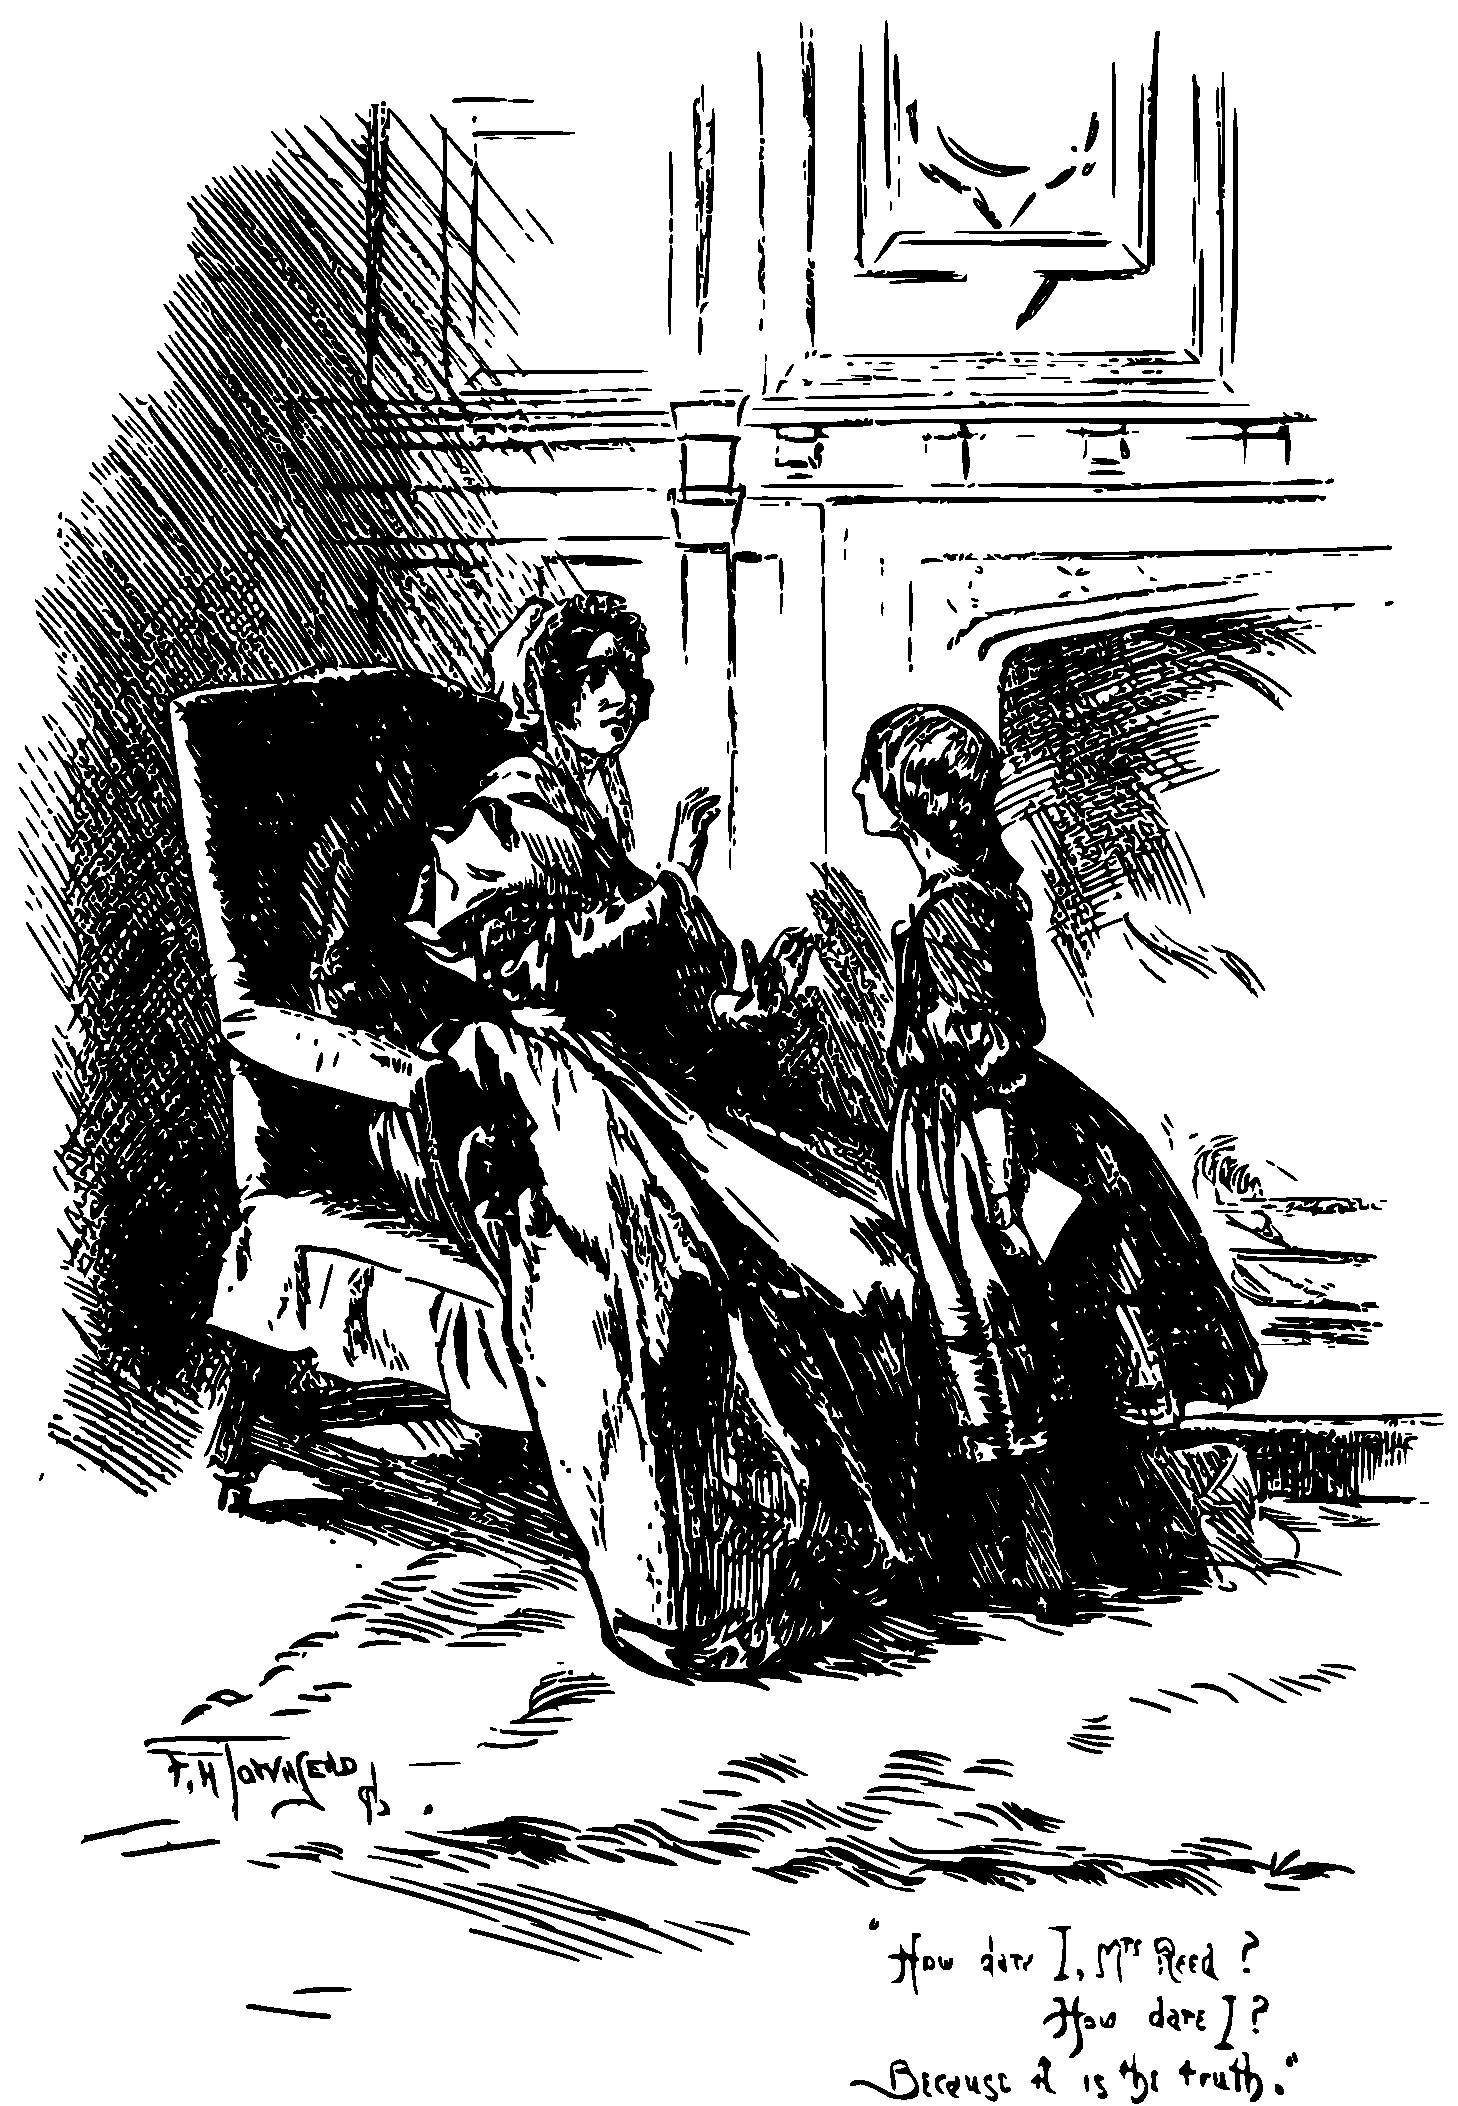
\includegraphics[width=\linewidth]{images/p30b.pdf}
	\end{sidecaption}
\end{figure}

Ere I had finished this reply, my soul began to expand, to exult, with
the strangest sense of freedom, of triumph, I ever felt. It seemed as
if an invisible bond had burst, and that I had struggled out into
unhoped-for liberty. Not without cause was this sentiment: \Mrs{} Reed
looked frightened; her work had slipped from her knee; she was lifting
up her hands, rocking herself to and fro, and even twisting her face as
if she would cry.

\enquote{Jane, you are under a mistake: what is the matter with you?
	Why do you tremble so violently? Would you like to drink some water?}

\enquote{No, \Mrs{} Reed.}

\enquote{Is there anything else you wish for, Jane? I assure you, I
	desire to be your friend.}

\enquote{Not you. You told \Mr{} Brocklehurst I had a bad character, a
	deceitful disposition; and I'll let everybody at Lowood know what you
	are, and what you have done.}

\enquote{Jane, you don't understand these things: children must be
	corrected for their faults.}

\enquote{Deceit is not my fault!} I cried out in a savage, high voice.

\enquote{But you are passionate, Jane, that you must allow: and now
	return to the nursery---there's a dear---and lie down a little.}

\enquote{I am not your dear; I cannot lie down: send me to school soon,
	\Mrs{} Reed, for I hate to live here.}

\enquote{I will indeed send her to school soon,} murmured \Mrs{} Reed
\emph{sotto voce}; and gathering up her work, she abruptly quitted the
apartment.

I was left there alone---winner of the field. It was the hardest battle
I had fought, and the first victory I had gained: I stood awhile on the
rug, where \Mr{} Brocklehurst had stood, and I enjoyed my conqueror's
solitude. First, I smiled to myself and felt elate; but this fierce
pleasure subsided in me as fast as did the accelerated throb of my
pulses. A child cannot quarrel with its elders, as I had done; cannot
give its furious feelings uncontrolled play, as I had given mine,
without experiencing afterwards the pang of remorse and the chill of
reaction. A ridge of lighted heath, alive, glancing, devouring, would
have been a meet emblem of my mind when I accused and menaced \Mrs{} Reed:
the same ridge, black and blasted after the flames are dead, would have
represented as meetly my subsequent condition, when half-an-hour's
silence and reflection had shown me the madness of my conduct, and the
dreariness of my hated and hating position.

Something of vengeance I had tasted for the first time; as aromatic wine
it seemed, on swallowing, warm and racy: its after-flavour, metallic and
corroding, gave me a sensation as if I had been poisoned. Willingly
would I now have gone and asked \Mrs{} Reed's pardon; but I knew, partly
from experience and partly from instinct, that was the way to make her
repulse me with double scorn, thereby re-exciting every turbulent
impulse of my nature.

I would fain exercise some better faculty than that of fierce speaking;
fain find nourishment for some less fiendish feeling than that of sombre
indignation. I took a book---some Arabian tales; I sat down and
endeavoured to read. I could make no sense of the subject; my own
thoughts swam always between me and the page I had usually found
fascinating. I opened the glass-door in the breakfast-room: the
shrubbery was quite still: the black frost reigned, unbroken by sun or
breeze, through the grounds. I covered my head and arms with the skirt
of my frock, and went out to walk in a part of the plantation which was
quite sequestrated; but I found no pleasure in the silent trees, the
falling fir-cones, the congealed relics of autumn, russet leaves, swept
by past winds in heaps, and now stiffened together. I leaned against a
gate, and looked into an empty field where no sheep were feeding, where
the short grass was nipped and blanched. It was a very grey day; a most
opaque sky, \enquote{onding on snaw,} canopied all; thence flakes felt
it intervals, which settled on the hard path and on the hoary lea
without melting. I stood, a wretched child enough, whispering to myself
over and over again, \enquote{What shall I do?---what shall I do?}

All at once I heard a clear voice call, \enquote{Miss Jane! where are
	you? Come to lunch!}

It was Bessie, I knew well enough; but I did not stir; her light step
came tripping down the path.

\enquote{You naughty little thing!} she said. \enquote{Why don't you
	come when you are called?}

Bessie's presence, compared with the thoughts over which I had been
brooding, seemed cheerful; even though, as usual, she was somewhat
cross. The fact is, after my conflict with and victory over \Mrs{} Reed,
I was not disposed to care much for the nursemaid's transitory anger;
and I \emph{was} disposed to bask in her youthful lightness of heart. I
just put my two arms round her and said, \enquote{Come, Bessie! don't
	scold.}

The action was more frank and fearless than any I was habituated to
indulge in: somehow it pleased her.

\enquote{You are a strange child, Miss Jane,} she said, as she looked
down at me; \enquote{a little roving, solitary thing: and you are going
	to school, I suppose?}

I nodded.

\enquote{And won't you be sorry to leave poor Bessie?}

\enquote{What does Bessie care for me? She is always scolding me.}

\enquote{Because you're such a queer, frightened, shy little thing. You
	should be bolder.}

\enquote{What! to get more knocks?}

\enquote{Nonsense! But you are rather put upon, that's certain. My
	mother said, when she came to see me last week, that she would not like
	a little one of her own to be in your place.---Now, come in, and I've
	some good news for you.}

\enquote{I don't think you have, Bessie.}

\enquote{Child! what do you mean? What sorrowful eyes you fix on me!
	Well, but Missis and the young ladies and Master John are going out to
	tea this afternoon, and you shall have tea with me. I'll ask cook to
	bake you a little cake, and then you shall help me to look over your
	drawers; for I am soon to pack your trunk. Missis intends you to leave
	Gateshead in a day or two, and you shall choose what toys you like to
	take with you.}

\enquote{Bessie, you must promise not to scold me any more till I go.}

\enquote{Well, I will; but mind you are a very good girl, and don't be
	afraid of me. Don't start when I chance to speak rather sharply; it's
	so provoking.}

\enquote{I don't think I shall ever be afraid of you again, Bessie,
	because I have got used to you, and I shall soon have another set of
	people to dread.}

\enquote{If you dread them they'll dislike you.}

\enquote{As you do, Bessie?}

\enquote{I don't dislike you, Miss; I believe I am fonder of you than of
	all the others.}

\enquote{You don't show it.}

\enquote{You little sharp thing! you've got quite a new way of talking.
	What makes you so venturesome and hardy?}

\enquote{Why, I shall soon be away from you, and besides}---I was going
to say something about what had passed between me and \Mrs{} Reed, but on
second thoughts I considered it better to remain silent on that head.

\enquote{And so you're glad to leave me?}

\enquote{Not at all, Bessie; indeed, just now I'm rather sorry.}

\enquote{Just now! and rather! How coolly my little lady says it! I dare say
	now if I were to ask you for a kiss you wouldn't give it me: you'd say
	you'd \emph{rather} not.}

\enquote{I'll kiss you and welcome: bend your head down.} Bessie
stooped; we mutually embraced, and I followed her into the house quite
comforted. That afternoon lapsed in peace and harmony; and in the
evening Bessie told me some of her most enchanting stories, and sang me
some of her sweetest songs. Even for me life had its gleams of
sunshine.
